
\documentclass{beamer}
\usepackage{amsmath}
\usepackage{graphicx}

\title{Absolute Maximum and Minimum of $f(x) = x^3$ on $[-2, 2]$}
\author{EE24BTECH11012 - Bhavanisankar G S}
\date{\today}

\begin{document}

\frame{\titlepage}

\begin{frame}
\frametitle{Question}
\textbf{Find the absolute maximum and minimum value of the function} $f(x) = x^3$ \textbf{in the interval} $[-2, 2]$.
\end{frame}

\begin{frame}
\frametitle{Theoretical Solution}
Given function: $y(x) = x^3$ \\[0.2cm]
First derivative: $y'(x) = 3x^2$ \\[0.2cm]
Second derivative: $y''(x) = 6x$ \\[0.2cm]
Critical points: Solve $y'(x) = 0 \Rightarrow 3x^2 = 0 \Rightarrow x = 0$ \\[0.2cm]
Edge values: $y(-2) = -8$, $y(0) = 0$, $y(2) = 8$ \\[0.2cm]
\textbf{Absolute Maximum:} $8$ at $x=2$ \\
\textbf{Absolute Minimum:} $-8$ at $x=-2$
\end{frame}

\begin{frame}
\frametitle{Computational Solution}
Using Gradient Ascent and Descent: \\[0.2cm]
Gradient Ascent: $x_{n+1} = x_n + \alpha f'(x_n) = x_n + 3\alpha x_n^2$ \\[0.2cm]
Gradient Descent: $x_{n+1} = x_n - \alpha f'(x_n) = x_n - 3\alpha x_n^2$ \\[0.2cm]
With $\alpha = 0.01$: \\
$x_{\text{min}} = -2$, $y_{\text{min}} = -8$ \\
$x_{\text{max}} = 2$, $y_{\text{max}} = 8$
\end{frame}

\begin{frame}
\frametitle{Graphical Representation}
\begin{center}
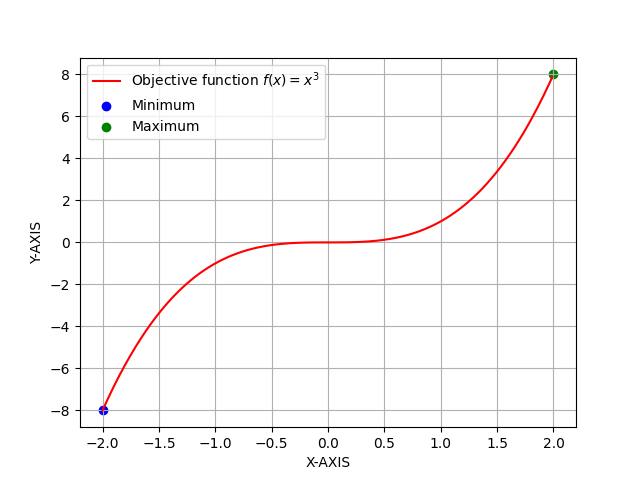
\includegraphics[width=0.7\textwidth]{fig.png} \\
\textit{Plot of the function $f(x) = x^3$ on $[-2, 2]$}
\end{center}
\end{frame}

\end{document}
